\chapter{Research}
\label{chp:research} 

\section{Related work}
In the last decade the importance of security against attacks on large computer systems has grown rapidly. In 2004, the ACM workshop on Visualization and data mining for computer security presented NVisionIP: netflow visualizations of system state for security situational awareness[kilde]. This was one of the first tools too visualize NetFlow data. The visualization was based on either number of bytes transmitted or the number of flows to or from the hosts on the network. 

In [Kilde] they discuss the use of NVisionIP to combat different security concerns. Most of the same attacks covered in this paper are relevant today, only in today's massive amounts of data, they may be way more difficult to discover. 

\begin{itemize}
\item \textbf{Worm infection}: One of the most basic security function one might uncover.  Worms usually spread by probing for other hosts. Filtering out hosts transmitting a lot of Flows with a single destination port, one could easily see which machines are infected and should be taken offline. 
\item \textbf{Compromised systems}: If a host is compromised, the attacker might install malware that allows the attacker to control the machine. Following this an attacker might turn a host into a file server. By detecting large volumes of traffic on certain ports one might discover such an attack. 
\item \textbf{Misuse}: Misuse of computer networks in order with terms of use etc.. An example is detecting if certain users have abnormal high volumes of traffic, and by inspecting in more detail one can uncover if this trough one single application and not in accordance with the policies of the organization. 
\item \textbf{Port Scans}: When a large number of ports are used at a specific host it is easily identified by NVisionIP.
\item \textbf{DoS}: Denial of Service Attacks will be visible trough spikes in traffic volume from the host attacking. If a host is attacked the same pattern is visible trough high volumes in receiving traffic. Thus peaks in traffic is not necessary an attack, but might be a result of a new release, or backup etc .. 
\end{itemize}

\section{Initial research}
In section[om netflow] we see how the raw format of the NetFlow packets look. Comparing how understandable this format is comparing to a visual representation will be the main object of this paper. How much more effective is visualization compared to the raw format read by machines. 

To understand this, experiments will determine how quickly one can distinguish an attack from both the raw format, and the visual representation. 

This is were D3.js will come to great use. It can be used to quickly develop simple interactive graphs that can be used to test up against each other.

To be able to identify an DDoS attack, one can look at it from two angles. By finding someone whom is attacking, or someone whom is being attacked. In this case we will look at the second scenario. As mentioned earlier simply a peak in flows is not enough grounds to establish an actual attack. First of all, one will need to look for patterns of similar incidents, and what lies behind them.

\section{Traits of a DDoS attack}
In a Distributed Denial of Service attack there are a large number of hosts performing the attack. In many cases a lot of them are not even aware they are a part on an attack. This is called a botnet, derived from the words robot and network. Using compromised systems, called zombies, gives the attacker control of a large enough amount of hosts to perform a volume-based DDoS attack. 

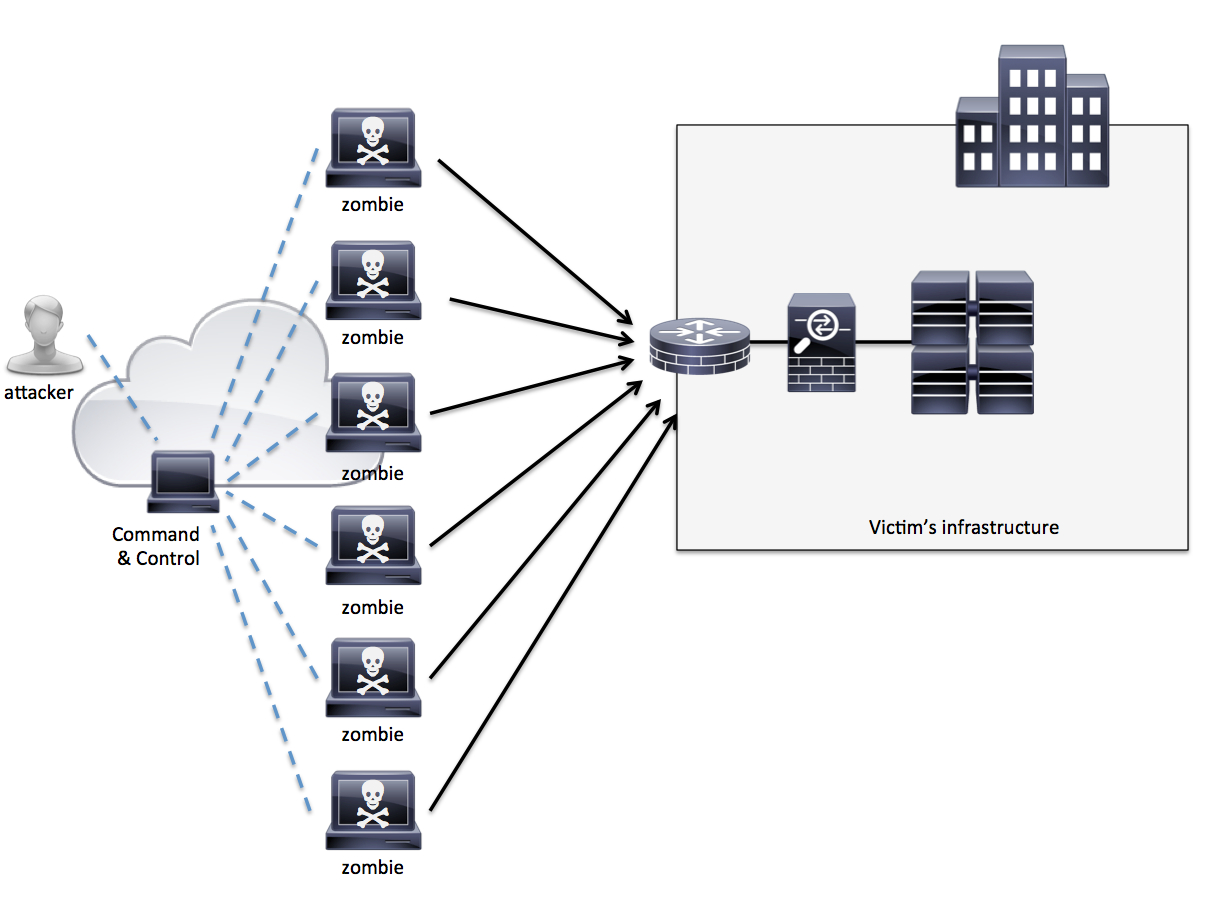
\includegraphics[scale=0.2]{botnet}

Another new trend that has emerged is using large datacenters or cloud machines to launch these attacks. Either trough renting or compromising them. As cloud providers are offering such large amounts of computers, this new platform is not only great for legitimate use, but also cyber-criminals.

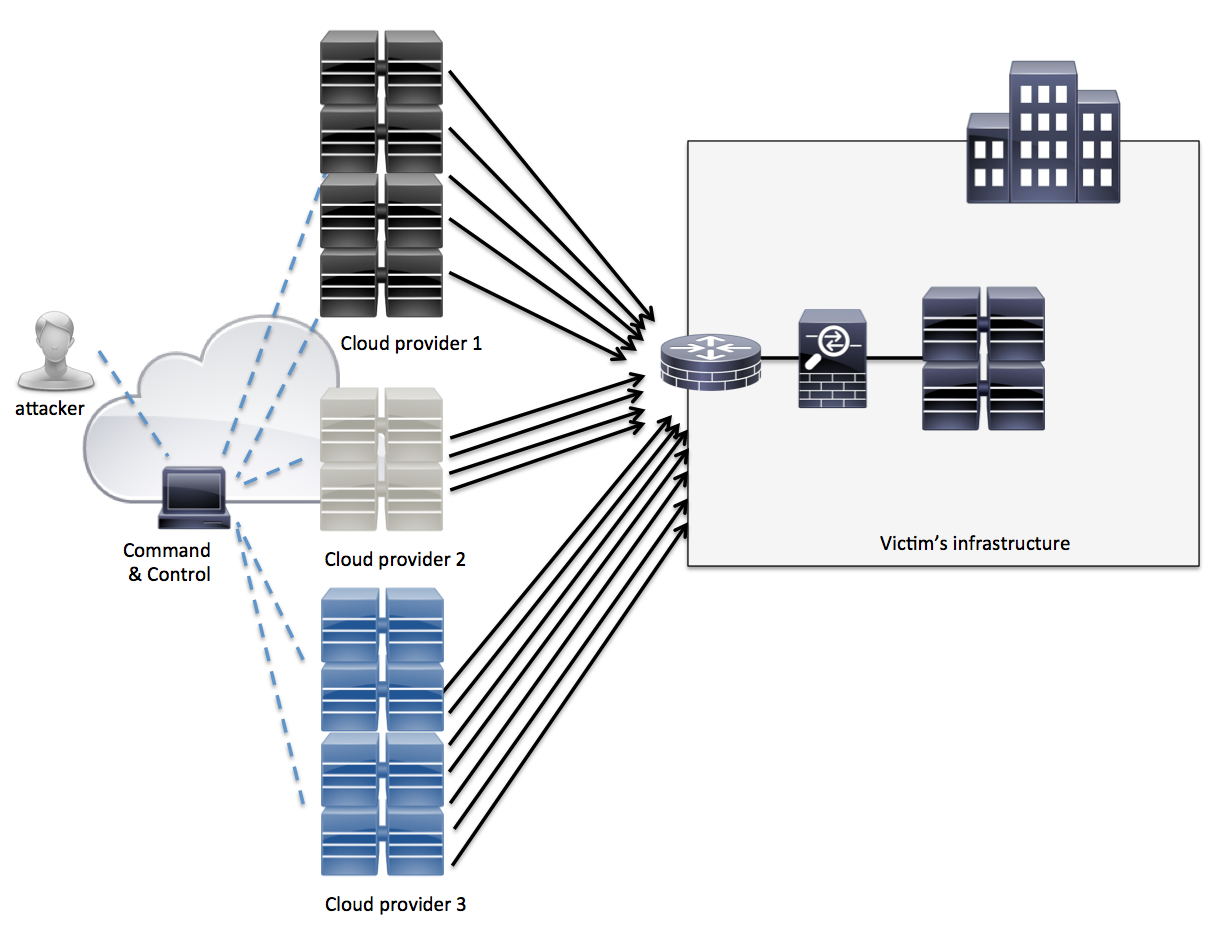
\includegraphics[scale=0.2]{cloud}

Distributed Reflection Denial of Service attacks is becoming more and more popular. DrDoS techniques usually involve mulitple victim host machines that unwillingly participate in a DDoS attack on the attackers primary target. Requests to the victim host machines are redirected, or re ected, from the victim hosts to the target. Anonymity is one advantage of the DrDoS attack method. In a DrDoS attack, the primary target appears to be directly attacked by the victim host servers, not the actual attacker. This approach is called spoo ng.
Ampli cation is another advantage of the DrDoS attack method. By involving multiple victim servers, the attacker’s initial request yields a response that is larger than what was sent, thus increasing the attack bandwidth.

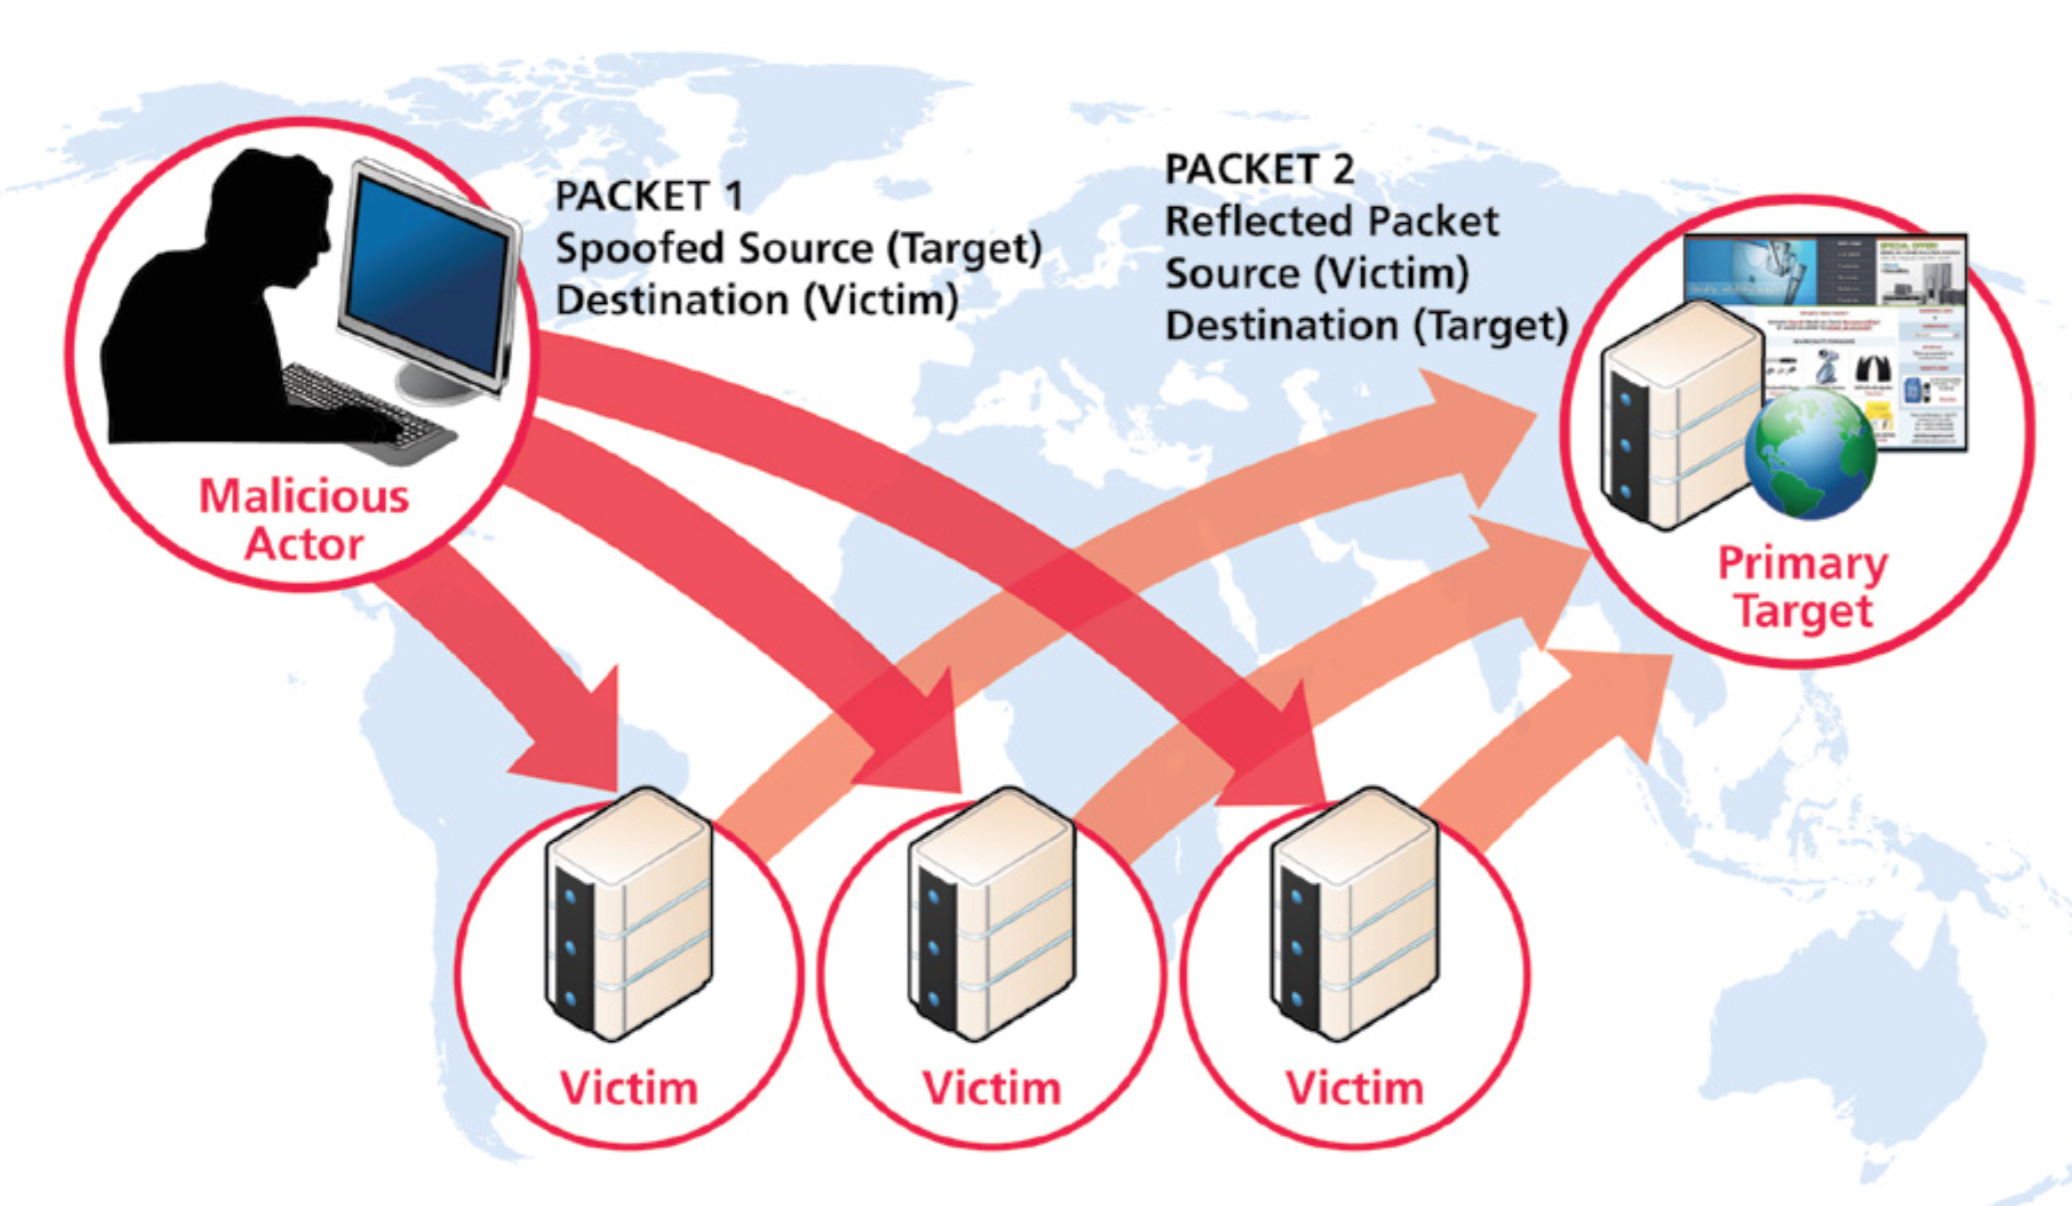
\includegraphics[scale=0.2]{drdos}

\subsection{Raw NetFlow format}
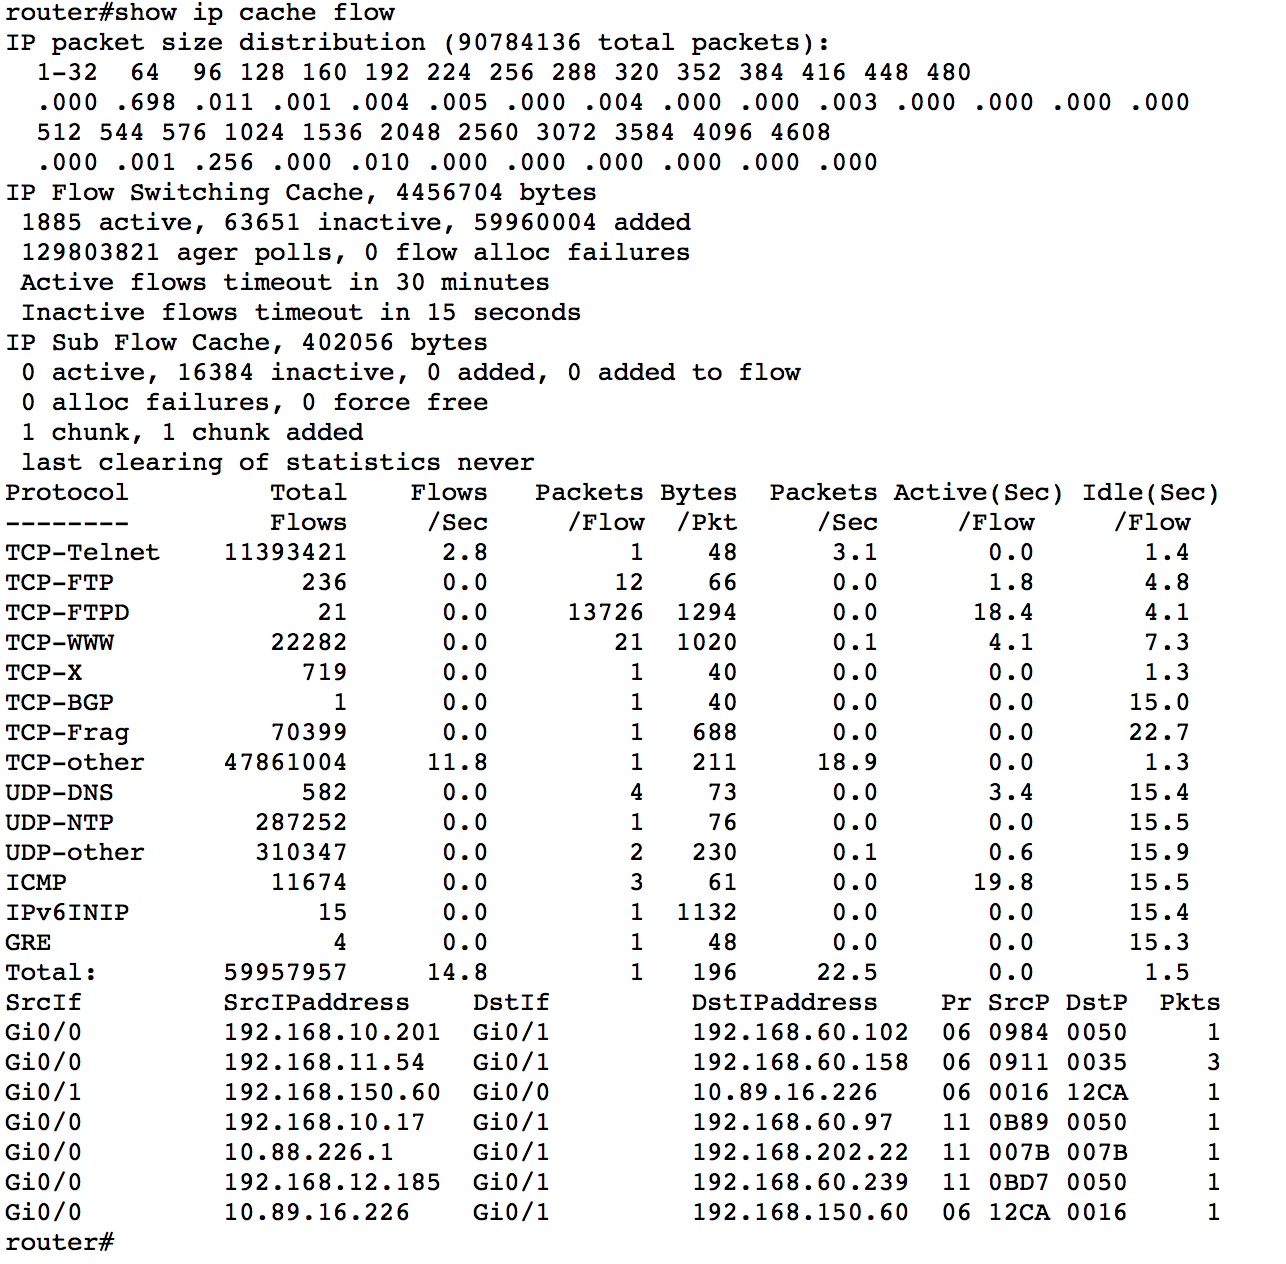
\includegraphics[scale=0.4]{netflow_ddos}
In the preceding example, there are multiple flows for UDP port 80 (hex value 0050). In addition, there are also flows for TCP port 53 (hex value 0035) and TCP port 80 (hex value 0050).

The packets in these flows may be spoofed and may indicate an attempt to perform these attacks. It is advisable to compare the flows for TCP port 53 (hex value 0035) and TCP port 80 (hex value 0050) to normal baselines to aid in determining whether an attack is in progress.

\todo{Finne kommandolinjeversjon av et DDoS angrep}


\section{Using D3.js}
Earlier in this paper it is mentioned that D3.js will be used to show examples of effective visualization of NetFlow data. It is assumed that the data has already been processed before it is made accessible to these examples. 

\subsection{Number of flows to a certain host and port}
This example shows how a simple graph can recognize a DDoS attack trough giving the option to see the number of netflows on different hosts and ports. 

\todo{Screenshot}

To confirm that such a solution is more effective, it must be tested. By creating a simple tool to convey information visually and give people with no or little information on NetFlow a chance to compare a visual solution to the raw machine readable data, and find out how effective it actually is.  

